\documentclass[sigplan,10pt]{acmart}
\renewcommand\footnotetextcopyrightpermission[1]{}
\pagestyle{plain}
\AtBeginDocument{%
  \providecommand\BibTeX{{%
    \normalfont B\kern-0.5em{\scshape i\kern-0.25em b}\kern-0.8em\TeX}}}
    
%%
%% end of the preamble, start of the body of the document source.
\begin{document}

%%
%% The "title" command has an optional parameter,
%% allowing the author to define a "short title" to be used in page headers.
\title{Trade-offs in slowing down network driven workloads}

\settopmatter{printfolios=true}

%%
%% This command processes the author and affiliation and title
%% information and builds the first part of the formatted document.
\maketitle

\section{Introduction}

\section{Experiment Setup}
%\section{Experiment Overview}
%% TODO JA - fill in your thoughts on why we picked these four specific workloads

In this section, we begin to narrate our study.
We present our chosen hardware platform and the three hardware parameters we explore (\S\ref{sec:knobs}, \S\ref{sec:exp_setup}),
detail our per-interrupt log collection methodology (\S\ref{sec:log_collect}),
briefly discuss our two target OSes and their configurations (\S\ref{sec:OS}),
and describe the application software and workloads we use to exercise this OS software (\S\ref{sec:apps}).

%% \begin{figure}
%%   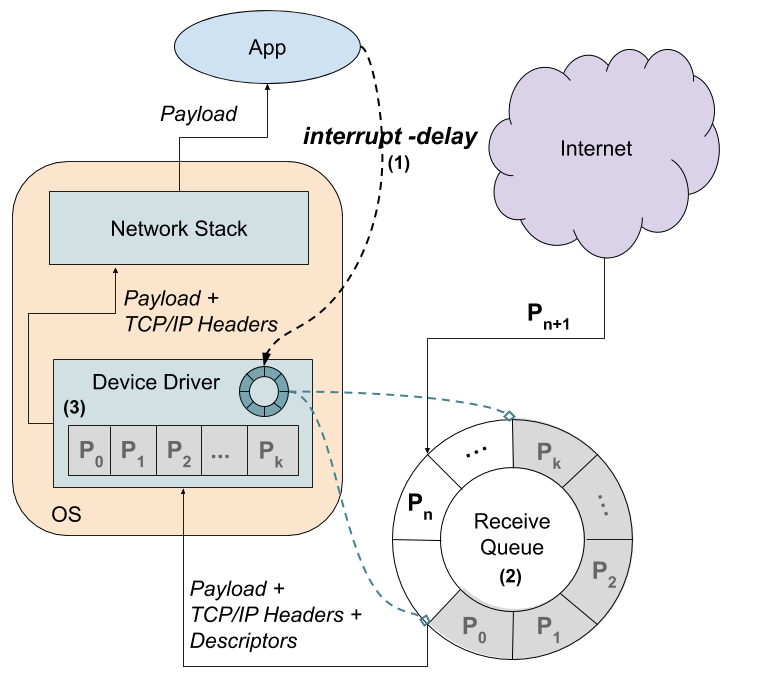
\includegraphics[width=7.7cm]{itr_figure.png}
%% \caption{As interrupt delay (1) is increased, the receive queue (2) buffers
%% more incoming packets as the NIC cannot fire new interrupts until the delay
%% value has been reached. Once the interrupt is fired, Linux's NAPI polling
%% mechanism kicks in and starts pulling in new packets (3) to be processed until
%% it either reaches its current work budget (calculated using existing jiffies)
%% or until there is no more data to be processed.}
%%   \label{fig:itr_figure}
%% \end{figure}

\subsection{Hardware Tuning Parameters}
\label{sec:knobs}
Below, we discuss the three hardware parameters studied,
outline Linux's default policies for tuning them,
and describe how we statically configure them. 

\subsubsection{NIC Interrupt Delay (ITR-delay)}
\label{sec:knobs_itr}
The Intel 82599 datasheet~\cite{82599}
defines a time-based interrupt throttling mechanism
which controls the delay (i.e. ITR-delay)
between fired NIC interrupts on target cores.
%The value of ITR-delay can range from \texttt{0} to \texttt{1024} \micro s
%and can be adjusted in increments of \texttt{2} \micro s.
%By default, Linux's network device driver uses a dynamic policy
%that seeks to tune ITR-delay to better reflect the resident workload between a range of 2 \micro s and 128 \micro s.
The policy collects data received from prior interrupts
about packet counts and bytes-per-packet
and uses it to classify the current state of the workload
(i.e. latency-critical or best-effort batch compute).
It then tunes ITR-delay accordingly
while abiding by pre-computed theoretical maximum wire speeds.

In Linux, the \textit{ethtool} program can be used
to statically set ITR-delay values
such that NIC interrupts fire at a fixed rate.
We take advantage of this ability in our study and tune ITR-delay values statically for different applications.
We focus on this NIC hardware setting
over thousands of others~\cite{82599}
due, firstly, to its ease of configurability in Linux (via \textit{ethtool}),
and secondly to its adoption by Linux's dynamic tuning policy
which we can use as a comparison point.


%Figure~\ref{fig:itr_figure} illustrates the interaction of interrupt delay
%values with the rest of systems software.
%The effect of setting a higher interrupt delay results in potential buffering
%of receive packets, thereby increasing packet processing efficiency at a
%potential cost to response time.

%received from the last interrupt and classifies them broadly into a set of
%ranges that are pre-computed based off theoretical maximum wire speeds.
%This delay tuning is applied upon the next interrupt occurrence.
%It is possible to disable this dynamic algorithm through the flip of a bit
%inside the device driver. After flipping this bit,


%device driver [REF] updates the interrupt delay value dynamically after every
%packet receive to a value based on the current traffic pattern. This value can
%also be fixed to a static value which results in interrupts being fired every X
%microseconds where X is a configurable value.


%To demonstrate its behavior, we instrumented a simple logging tool into the
%IXGBE device driver.
%Figure~\ref{fig:itr_delays} shows a small snapshot of its values while running
%a Memcached workload.
%Each marker represents a new \textit{ITR-Delay} value.
%In its current implementation, it can only seek values between the range of 2
%to 126 microseconds.
%The reason for this is that it was never designed towards a use case of
%aggressively delaying packet receive interrupts to take advantage of energy
%proportionality under stringent SLAs, which can potentially result in setting
%\textit{ITR-Delay} values in the hundreds of microseconds.

%It is also possible to disable this dynamic algorithm through the flip of a
%bit inside the device driver.
%This requires a rebuild of the driver module as it was not a configurable
%parameter.
%After flipping this bit, we can use Linux's \textit{ethtool} to set new
%interrupt delay values statically to fire every X microseconds, where X is a
%configurable value.


\subsubsection{Running Average Power Limit (RAPL)}
\label{sec:knobs_rapl}
RAPL~\cite{intel_rapl} is a power limiting feature on Intel processors
that can be used to throttle power-draw of different hardware components.
It's utility has been investigated~\cite{rapl2015, rapl2018, PerAppPower},
quantifying its accuracy and low performance overhead
while illustrating per-workload power constraints.
In our experiments, we use the RAPL model specific registers (MSR) to explicitly set power limits up to a default maximum of 135 Watts
in a single package on our 2-package processor. After some initial experimentation, we
found that our workloads continue to execute correctly at a minimum RAPL limiting value of around \texttt{55}.
%When applying power limits, care must be taken to ensure
%there is a minimum RAPL value such that an application's continued execution
%can be sustained in this limited power budget.
%Applications often depend on hardware components that in turn rely on a
%minimum power supply to continue running.
%Hence, when considering energy efficient compute, calculating minimum RAPL
%values that would sustain the execution of a particular workload becomes
%important.
%After some initial experimentation,
%5we found that our class of workloads continues to execute correctly
%at a minimum RAPL limiting value of around \texttt{55} \watt.


\subsubsection{Dynamic Voltage/Frequency Scaling (DVFS)}
\label{sec:knobs_dvfs}
We use the term DVFS~\cite{cpufreq_governor} to describe the ability to set the processor's frequency.
Linux by default contains a dynamic policy to adjust based on current processing load.
Through experimentation, we found Linux's dynamic policy uses a range between
a min frequency of \textbf{0xc00} and a max of \textbf{0x1D00}. We use this range of settings in our study

%DVFS~\cite{cpufreq_governor} is an energy tuning dynamic policy,
%built into Linux,
%that dynamically adjusts voltage/frequency operating points (P-states)
%on individual cores
%based on current processor load.
%Intel power states (p-states) is another energy saving
%feature on Intel processors.
%It allows users to set specific p-states for individual cores.
%A p-state is a combination of the clock frequency and voltage that a core is
%operating on.
%Typically,  p-states are set dynamically according to current
%processor load by a policy governor in Linux called Dynamic Voltage Frequency
%Scaling (DVFS).
%DVFS can be disabled,
%enabling static configuration of P-states
%by updating the IA32\_PERF\_CTL Intel register~\cite{intel_msr}.
%A p-state is the combination of a core's clock frequency and its voltage at
%some ratio, however, it is unclear how it exactly translates to real processor frequency.
%When setting up our experiments,
%we monitored the MSR\_PERF\_STATUS register~\cite{intel_msr}
%and found that the range of values set by Linux's DVFS policy
%starts with a minimum of \texttt{0xC00}
%and ends with a maximum of \texttt{0x1D00}.
%We use this range of settings in our study
%to statically tune processor P-states
%in both Linux and our library OS.


\subsection{Hardware Platform}
\label{sec:exp_setup}
Our experimental cluster consists of seven nodes,
each having 16-core processors of either 
Intel(R) Xeon(R) CPU E5-2690 @2.90GHz
or Intel(R) Xeon(R) CPU E5-2650 @2.60GHz type.
All processors have Intel Corporation 82599ES 10-Gigabit SFI/SFP+ NICs,
and all nodes are configured with a mix of 126 GB and 250 GB RAM.
The node we use to boot into our baremetal library OS and Linux
contains an Intel(R) Xeon(R) CPU E5-2690 @2.90GHz processor
with 126 GB of RAM.

When running our experiments,
we ensure that the processors hosting Linux and the library OS
are setup as similarly as possible.
We carefully configure IA-32 Architectural MSRs and processor specific MSRs
(see Tables 35-2 and 35-18 in ~\cite{intel_msr})
as well as NIC features:
direct-cache injection (DCA) disabled,
receive-side scaling (RSS) enabled
(to distribute packets for multi-core processing),
and hardware checksum offloading enabled.
We also match the values of
the number of NIC transmit and receive descriptors
and write-back thresholds for packet transmissions.
Additionally, to minimize system noise,
we disable hyperthreads and Turbo Boost features on all processors.


\subsection{Per-interrupt Log Collection}
\label{sec:log_collect}
%NAPI?

%In order to better understand the interactions of ITR, DVFS, and
%RAPL with a server that is under some load, we instrumented \textit{fine-grained per-interrupt} log collection in both Linux and libOS' network device
%driver on the interrupt handling path.
%In order to reveal novel information
%about the interactions between the OS, application workloads, and hardware
%under different energy profiles,
%we find that it is constructive to place hardware events,
%such as transitions in C-states and network I/O events,
%on some form of timeline.
%When such a temporal construct is backed by detailed experimental logs,
%it allows us to draw conclusions about the impact of OS software
%on full system execution: performance and power-draw.
%It enables us to locate and analyze relevant power-events
%in the span of execution of a workload that can be attributed
%either to the involvement of OS software
%to maintain energy proportionality
%or lack thereof.

To study and effectively identify the role of the OS
in affecting the global energy-performance behaviour,
we found it critical to use an interrupt-centric methodology.
This is because the OS interrupt and polling behavior partitions time
into busy and idle periods,
whereby the OS controls energy consumption behavior during idle time
while its design and implementation have a significant impact
on the instructions that compose busy time and their efficiency.
As such,
we found that local behavior of the OS, demarked between interrupts,
combines to significantly influence global system behavior and performance.
Interrupt-centric energy-performance logs
enable us to locate and analyze relevant power events
in the span of execution of a workload.
These events can be attributed
either to the involvement of OS software to maintain energy proportionality
or lack thereof.
Typical logging approaches,
such as periodic PC sampling,
can overlook these critical OS episodes.


Motivated by this rationale,
we designed an interrupt-centric data collection methodology
that gathers fine-grain per-interrupt logs
of hardware statistics relevant to
the performance and energy profile
of a particular workload
and of the system overall
\footnote{
To ensure minimal overhead by our logging mechanism,
we use non-temporal store instructions to store collected statistics
into an in-memory array
%We found that using non-temporal store instructions had more of an impact on
%the performance of EbbRT versus that of Linux.
%We believe that this could be due to the fact that EbbRT was built to be an
%efficient library OS and hence its performance is more observably affected by
%additional logging.
}.
As we target network-bound workloads,
we decide log data at the event of NIC receive and transmit interrupts.
We collect the following information at every interrupt:
received and transmitted bytes,
the current timestamp (via the \texttt{rdtsc} instruction),
and various sleep state statistics.
We also collect a set of hardware statistics
from per-core performance monitoring counters (PMCs)
at a maximum granularity of 1 millisecond\footnote{
The MSR\_PKG\_ENERGY\_STATUS register allows software to query the energy consumption (in Joules) of a specific package. It conforms to a maximimum sampling frequency of 1 millisecond. Hence we only read from PCMs when the time elapsed between interrupts is at least 1 millisecond.
}:
instructions, cycles, last-level-cache misses, and the energy consumed,
which we read from the MSR\_PKG\_ENERGY\_STATUS register.
This set of statistics also helps us
take a detailed look at the per-core behavior
while acquiring a global perspective on overall resource usage
when hardware settings are tuned in different ways (\S\ref{sec:knobs}).

Our use of fine-grain interrupt-centric data logging
has allowed us to break-down and analyze OS behaviours in our library OS
that causally contribute to its realized energy-performance profile.
We describe some of these behaviors in Section \S\ref{sec:OS_libos} 
and refer to them throughout our analysis of experimental data
(see Section\S\ref{sec:analysis}).




%While this data provides a breadth of directions to reason about the results
%below, we discovered that it can be helpful to focus on subsets of data points
%for different workloads.
%\subsubsection{Measurements}
%\label{sec:measures}
%\begin{itemize}
%       \item Throughput and Latency: Throughput is defined to be the
%time-average of total data transferred. It is measured in units of
%[bytes/second].
%         Latency is a measure of the delay between a request and the
%corresponding response. It is measured in [seconds]. Due to the stochastic
%nature of latency, we follow the convention of measuring the 99th percentile of
%the latency distribution for multiple requests.
%Depending on the workload, either throughput or latency is a direct measure of
%network %performance.
         %[Any notes about exact measurement process?]
       %\item Energy and Power
    %     [Note about Joule counter]
         
     %  \item Instructions, Cycles, Cache-Misses
	%\item Device Driver Statistics
	%\item Sleep States
%\end{itemize}


%\subsection{Experimental Setup}


\subsection{OS Software}
\label{sec:OS}
As noted, we run our experiments using
Linux and a libOS, both running baremetal.
%We use a statically configured libOS,
%a statically configured build of Linux,
%and a build of Linux that uses default power management mechanisms.
We adjust the above hardware settings statically in the libOS and Linux and compare
against default Linux with its dynamic policies enabled.
In our figures and analysis,
we refer to these OSes as \textit{LibOS tuned},
\textit{Linux tuned}, and \textit{Linux default}, respectively.


\subsubsection{Linux}
\label{sec:OS_linux}
In order to ensure a fair comparison our single-purpose library OS and general-purpose Linux, we build a set of application-specific Linux \textit{appliances} for our four workloads. Reminiscent of library OSes~\cite{unikernels}, these appliances are specially constructed to run a RAM-based filesystem and contain only a small set of system libraries and kernel modules required to run their constituent applications. We construct these appliances from a base Debian 10.4 distirbution and use a custom 5.5.17 kernel which we build using a modified configuration file created for supporting high performance, following suggestions from previous work that studies Linux core operation costs~\cite{linux-core-ops}. To avoid scheduling overheads and noise, we pin all applications to physical cores. In addition, we disable Linux ~\textit{irqbalance} and affinitize packet receive interrupts to their respective cores.

Given the general-purpose nature of Linux, it contains many policies and mechanisms that interact with overall application and system execution. For example, it contains the CPU Idle Time Management Subsystem which comprises logic integrated into various parts of the system in order to manage when and how to idle. The subsystem itself decomposes further into selectable {\tt CPU idle} governors, of which we use the recommended {\tt intel\_idle} governor to exploit the Intel-specific multi-level sleep states (C1, C1E, C3 and C7). Linux also encorporates NAPI~\cite{napi}, which interacts with the detection and dispatching of network packets for balancing poll and interrupt-driven operation of the network device.

%It determines when and how to sleep the processor
%based on system load measurements
%and predictions of interrupt occurrence times.
%See \cite{orran_NIC_paper} for an overview of how the
%device driver for our network card interoperates with the rest of the
%Linux networking subsystem (including its management of the ITR
%value).

All of these performance management components are entangled deeply in Linux's design and implementation, making it difficult to pin down how they interact with each other and with the rest of the system. For example, predicting the time of occurrence of the next interrupt relies on gathering device-level interrupt activity and wake-up statistics and hence interacts with the layered generic interrupt management subsystem of Linux. Moreover, ITR-delay changes can influence NAPI and idle management behavior, which together can affect the selected halt states and the net influence of DVFS and RAPL settings.

We posit that application execution can benefit greatly from eliminating the interference and overhead of dynamic policies and mechanisms. In our study, we explore static hardware configurations of performance settings in detail (see \S\ref{sec:knobs} for a quantification of explored values) with the goal of unveiling 1) any headroom that exists for improving the overall performance and energy consumption of application-workloads in Linux and 2) insight about the interaction of these workloads with the system software.


%Describe details of configurations considered and various policies and
%mechanisms we know our workloads interact with.  Eg.  device driver, itr, napi,
%idle sleep states, etc. Also discuss what app software used.
%upon execution of the \texttt{halt} instruction\footnote{
%The sleep state logic was developed
%based on the \texttt{intel\_idle} functionality in Linux.
%}.

\subsubsection{Library OS}
\label{sec:OS_libos}
We use an existing libOS with specialized components\footnote{ All components are multi-core functional and optimized to aggressively use per-core memory and fine grain locking.}, including a NIC driver, a custom TCP/IP stack, virtual and physical memory allocators\footnote{Memory allocators make aggressive use of large pages and pinned memory to avoid page-faults.}, and a generic I/O buffer\footnote{I/O buffers are designed to enable zero-copy application data processing.} The library OS is packaged as a library of configurable modules and \textit{gcc-5.3.0}-based tool-chain targeting the base components of the OS. 

Applications are ported to it by configuring the necessary OS components and compiling the application source along with any dependent libraries using this tool-chain. This process generates a single application-specific binary that is source and link-optimized with the OS code. Prior studies have indicated the benefits of both compile-time and link-time optimization on library OS function dispatching~\cite{ebbrt}. We built a baremetal port of the libOS by writing a network device driver for the Intel 82599 NIC. Our bare-metal port enables application-specific binaries to boot directly on our hardware platform. Once booted, OS and application code is executed under a single supervisor privilege domain. The library OS strictly adopts a run-to-completion, event-driven execution model\footnote{All event handlers are run with interrupts disabled and are expected to return back to the event loop.} and bears similarity to other library OSes designed for high-performance network services\cite{ix,seda,arrakis,ebbrt}. 

Given the design and implementation for single-application, non-preemptive processing via an optimized OS and application binary, the library OS components can avoid many checks and streamline execution, ranging from interrupt dispatch to application logic. The NIC device driver totals over 3000 lines of code and interfaces with the library OS multicore TCP/IP network stack\footnote{The device driver programs the NIC using per-cpu queues and interrupts, maintaining the affinity of TCP connections to their respective cores.}. It inherently does not have a dynamic policy for updating ITR-delay values, but does provide an interface for statically setting them. We use this interface in our study as we sweep across hardware parameter values. 

The baremetal library OS follows a simple implementation and idling behavior. If no interrupt events or software events exist, the event-loop of the library OS infers that the system is idle and halts the core to enter the deepest sleep state supported by our hardware (C7). In contrast, upon receiving a packet, the device driver management code, protocol processing code, and application code can be dispatched and run to completion on a single event triggered by a NIC interrupt. The NIC driver also exposes a configurable constant (set to 64 for all our experiments) that is used to control how many packets can be processed in a single interrupt invocation before returning to the event-loop of the core on which the interrupt was processed. This behaviour, in turn, introduces a simple bounded per-cpu device-level poll. The libOS idling and device-polling policies are simple compared to Linux policies. %Our study reveals the contrast between these library OS policies and those applied by Linux through presenting a detailed quantification of execution trends and power events. It uncovers surprising impacts of OS functionality on overall system execution and yields insight on OS-level adaptations for energy-performance goals.


%-----------------------------
%
%IN PROGRESS
%
%-----------------------------
%
%\textit{
%\begin{description}
%\item[F3: Energy adaptation] As many have observed there is a tension between using controls to throttle processing and thus energy consumption versus the saving that can be had by finishing work quick and halting into lower energy consuming processor sleep states between the requests for work.  The later strategy is often referred to as "race-to-halt" (r2h) while we will refer to the former as "slow-to-stay-busy" (s2sb).  We found that these behaviours, and their effectiveness are largely emergent due to interactions between various interrupt and polling mechanisms and policies.  Additionally, we find that it is possible for a system to effectively modulate between both and that this ability allows the OS to again exploit a wider range of hardware settings over which behaviour can be optimized.  
%\item[F4: Virtuous Interactions] While it can be very hard to predict how the various hardware setting and software policy modules will interact, there can exist virtuous relationships that can be exploited.    A system has many different settings and behaviours that directly on indirectly affect the energy-performance profile.  It is natural in a complex OS for a set of mechanisms and policies to be constructed for a particular category of hardware settings.  Case-in-point being the sleep state that the processor will enter into on execution of the halt instruction.  Our processor defines several such states, each offering a different tradeoff in power consumption and penalties for entry and exit.  Not surprisingly, several mechanism in Linux interoperate to estimate when to halt and to what sleep state -- including work on the interrupt path used to create an estimate of interrupt arrival and the load induced.  We found, however, that if your OS paths are simple then a fixed halt to deepest sleep state and poll strategy can be sufficient.  The penalty of using the deepest sleep state can be mitigated by modulating the number of halts required by using the processor's throttling controls.   This in turn means that you need not have the complexity added complexity of sleep state management making your system simpler and reducing the number of control points.  But of course to do this you must have the headroom in processing done on every interrupt.   We believe other such opportunities exist ...
%\end{description}
%}

%this is partly due to the fact that Linux's dynamic
%ITR delay policy relies on  NAPI polling budgets which the libOS does not.

%todo: JA this is wrong we do not fire an periodic interrupt to force processing
%.     The RCU garbage collector is not for the driving of event processing
%As our library OS follows an event-driven model, whereby on each core, an
%interrupt is fired after every static period of time to check a list for new
%events to process;

%See~\ref{ref:ebbrt} for more details regarding the library OS. 


\begin{table}[t]
\centering
\begin{tabular}{l|c|c|c}
  Name & Scenarios & Nature & CPU\\
  \hline
  NetPIPE & {\small 64B,8KB,64KB,512KB} & CL & Low\\ \hline
  NodeJS & na & CL & High \\ \hline
  Memcached & 200K, 400K, 600K & OL & Low \\ \hline
  Memcached-Silo & 50K, 100K, 200K & OL & High \\ 
\end{tabular}
\caption{Workload configurations.
%NetPIPE and NodeJS are single thread, single connection, closed-loop (CL) workloads. Memcached and Memcached-silo are multiple core, multiple connection, open-loop (OL) workloads.
The column {\em Nature} indicates open-versus-closed loop nature
and {\em CPU} indicates application CPU demand.}
\label{table:wrkcfgs}	
\end{table}

% \subsection{Application Software and Workloads}
% \label{sec:apps}
% %      \begin{figure*}
        \centering
        \begin{subfigure}[b]{0.34\textwidth}
            \centering
            \caption[]%
            {{\small Netpipe}}  
            \vspace*{-0.3cm}  
            \label{fig:perf_netpipe}
            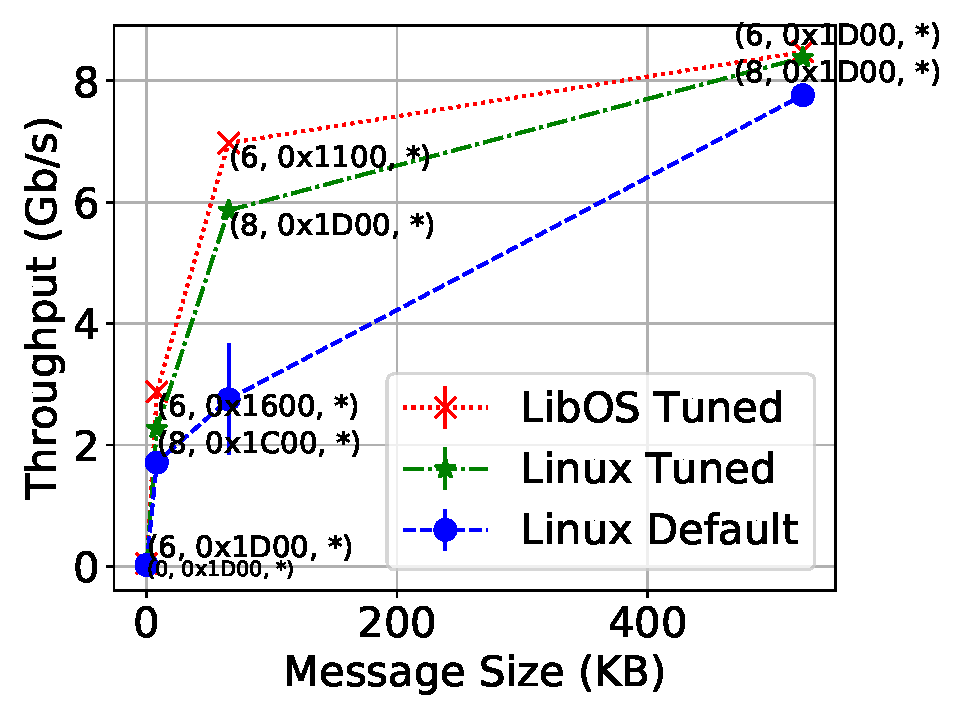
\includegraphics[width=1\textwidth]{osdi_figures/netpipe_tput}
        \end{subfigure}
 %      \hfill
        \begin{subfigure}[b]{0.32\textwidth}  
            \centering 
            \caption[]%
            {{\small Memcached}} 
            \vspace*{-0.3cm}    
            \label{fig:perf_mcd}
            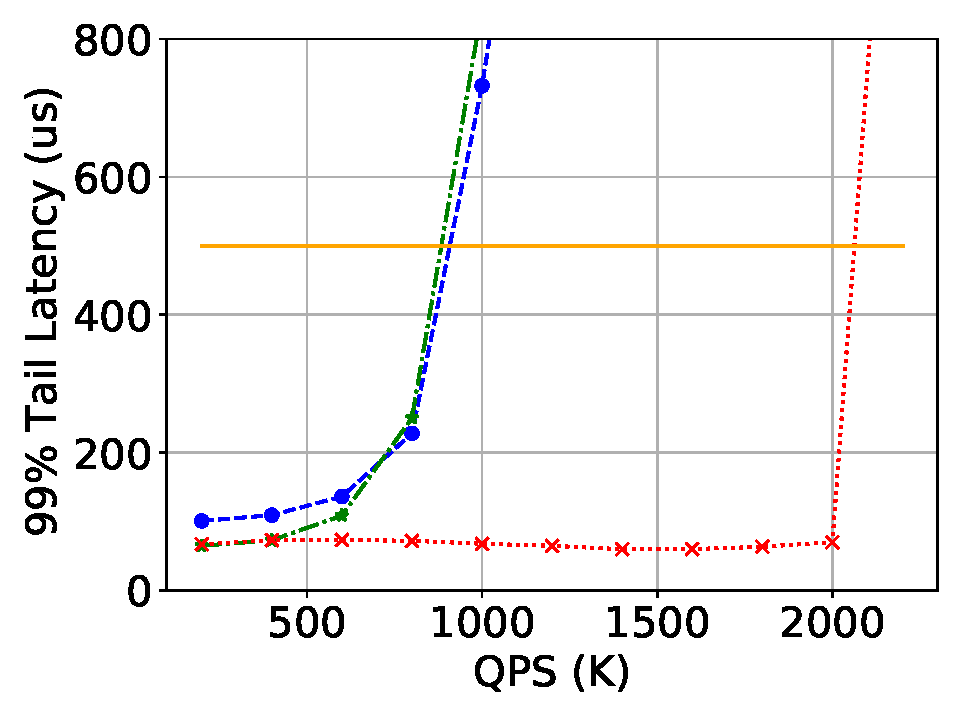
\includegraphics[width=1\textwidth]{osdi_figures/mcd_sla.pdf}
        \end{subfigure}
 %      \hfill
 %     \hspace{0.8cm}
        \begin{subfigure}[b]{0.32\textwidth}   
            \centering 
            \caption[]%
            {{\small Memcached-silo}} 
             \vspace*{-0.3cm}     
            \label{fig:perf_mcdsilo}
            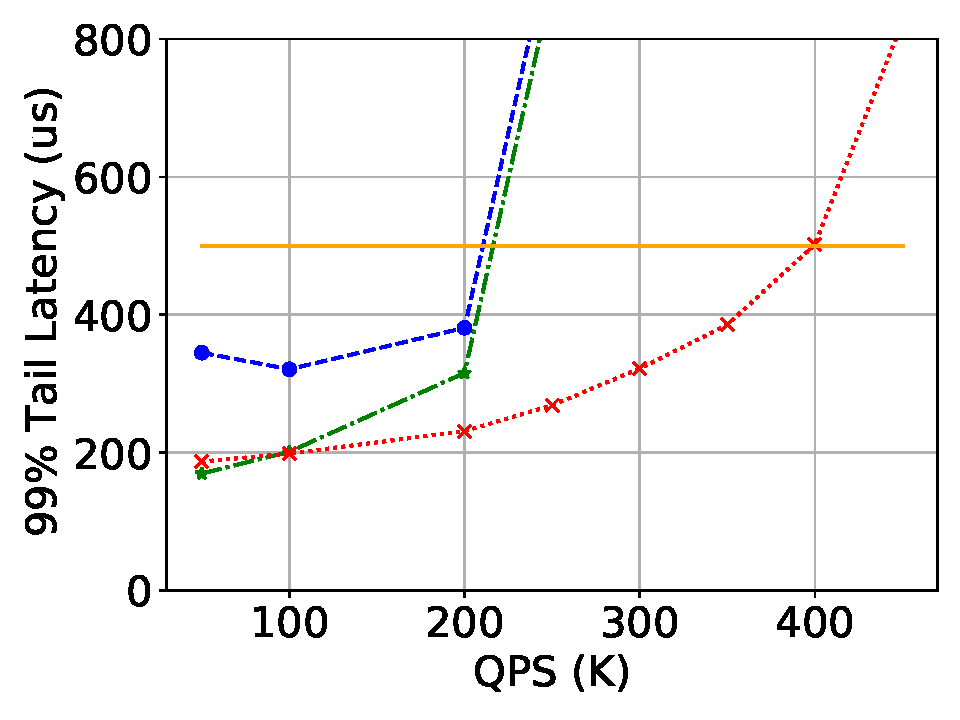
\includegraphics[width=1\textwidth]{osdi_figures/mcdsilo_sla.pdf}
        \end{subfigure}
        %\vspace*{0.3cm}  
        \caption[]
        {\small Performance baselines for NetPIPE across message sizes (64 B, 8 KB, 64 KB, and 512 KB) and  Memcached and Memcached-silo across different QPS rates.
For netpipe, the standard deviation around mean throughput is shown
for each message size.
The orange lines in both Memcached plots indicate an SLA objective of 500 {\micro}s.} 
        \label{fig:perf}
    \end{figure*}

% In this subsection, we describe in greater detail the four network-bound workloads that we target and their respective attributes. We present netpipe and nodejs as closed-loop experiments due to the fact that their performance (i.e. throughput) is dependent on the responsiveness of constituent server and client threads. In contrast, we present memcached and memcached-silo as open-loop experiments, as their performance boils down to the ability of their server threads to maintain a 99\% response tail latency under 500 {\micro}s under some offered load. Netpipe and memcached are OS-centric workloads by virtue of their computationally light application logic and reliance on OS functionality. In contrast, nodejs and memcached-silo as application-centric workloads, as their runtime and application logic are more computationally intensive.

% \subsubsection{NetPIPE}
% NetPIPE~\cite{snell1996netpipe} 
% involves sending messages of identical size between two systems via a single network connection for a fixed number of iterations. We fix the iteration count at 5000 and show results for a range of message sizes\footnote{We found that the 10 GB link is close to saturation when a message of size greater 700 KB is exchanged.}.

% %Using various message sizes with the netpipe application and configuring both sides with the same OS and hardware parameters allows one to expose the OS impacts on network communications in a controlled fashion.

% \subsubsection{NodeJS}

% NodeJS~\cite{nodejs} runs a JavaScript HTTP Webserver and consists of a single client, running the \textit{wrk}~\cite{wrk} benchmark\footnote{We modified \textit{wrk} to place a fixed request load of 100K.}, that sends web requests to a server thread for a fixed period of time via a single network connection. The server responds to each request with a small static payload of size 148 bytes. The library OS was ported to support baremetal NodeJS by providing OS interfaces that link with the V8~\cite{v8} JavaScript engine and libuv~\cite{libuv}.

% %In contrast to netpipe, the workload is not fixed and performance is measured
% %in requests-per-second once the benchmark has finished running. Further, a
% %nodejs web server is computationally heavier than netpipe.

% \subsubsection{Memcached}
% Memcached~\cite{mcd} is a multi-threaded workload that runs on all 16 cores of any one of our server nodes. It consists of an unloaded client node running mutilate~\cite{mutilate}. This client (1) coordinates with five other mutilate agent nodes in order to generate requests to the server and (2) measures tail latency of all requests made. All five agent nodes are 16-core machines, whereby each core creates 16 connections, for a total of 1280 connections. This setup is able to saturate the single 16-core server\footnote{Mutilate is configured to pipeline up to four connections to further increase its request rate.}. Our library OS uses a re-implemented version of memcached, written to the OS's interfaces, which supports the standard memcached binary protocol. To alleviate lock contention, an RCU hashtable is used to store key-value pairs. We run a representative load from Facebook~\cite{workloadanalysisfacebook} (ETC) which represents the highest capacity deployment. It uses 20 - 70 byte keys and 1 byte to 1 KB values and contains 75\% GET requests.

% %While the library OS's implementation does lack some additional features,
% %such as authentication and other commands,
% %it is functional enough to support the mutilate benchmark.

% \subsubsection{Memcached-Silo}
% Memcached-silo~\cite{mcdsilo, zygos} is a workload built on top of the normal memcached protocol. It is computationally complex as it encorporates both latency-sensitive network compute and memory-intensive TPC-C style transaction processing. We port the memcached-silo implementation to our library OS. The configuration and SLA constraints of memcached-silo follow from those of memcached. Given its computationally heavier nature, we only needed two 16-core server nodes at 16 connections per core to saturate our memcached-silo server.


% \subsection{Hardware Parameter Sweeping}
% \label{sec:hw_tuning}
% Section~\ref{sec:knobs} lists the ranges of values with which we tune hardware parameters. For each application, we further reduce the set of thse values based on small experiments that we run a priori. This experimental customization allows us to ensure that (1) increasing ITR-delay and lowering DVFS processor frequency does not bring about SLA violations for the memcached applications, and (2) lowering RAPL power limits does not cause the application and/or overall system to crash. Table~\ref{table:wrkcfgs} lists all different hardware configurations for every target workload. For NodeJS, Memcached, and Memcached-Silo, we apply hardware configuration on the server side only. For all target hardware configurations, we repeat every experiment 10 times to ensure statistical stability. \textbf{Netpipe}: We select four representative message sizes (64B, 8KB, 64KB, and 512KB) with a fixed round trip of 5000 iterations.  As NetPIPE consists of the same binary running as a client and a server, we configure ITR-delay to be the same in both client and server nodes. \textbf{NodeJS}: We use the \textit{wrk}~\cite{wrk} benchmark to place load on the nodejs server with 100K requests. \textbf{Memcached}: We use Mutilate~\cite{mutilate} to generate three different requests-per-second (QPS) rates of 200K, 400K and 600K, for a fixed period of 20 seconds each. \textbf{Memcached-Silo}: We use lower QPS rates of 50K, 100K, and 200K to account for increased computational load per request.

% \subsection{Performance Baselines}
% In order to create a context for analyzing our experimental results, we initially run the workloads in a more traditional manner: under hardware configurations that yield the best performance independent of energy consumption. For workloads running in tuned Linux and our library OS, we identify these performance-centric hardware configurations during our sweep of parameter values. This step is critical for establishing baseline energy-performance profiles for the different OS/workload pairs. Such baselines provide our study with relevant comparison points.

% %In order to put the results of our energy study into context we run
% %the workloads on the three OS configurations, Linux Default, Linux Tuned
% %and the library OS, in a more traditional manner to establish baseline
% %performance for each.  
% %For Linux tuned and the library OS we use our sweep data to identify, for each system, the hardware settings that yield the best performance independent of energy consumption for each of the message sizes.  
% \textbf{NetPIPE:} Figure~\ref{fig:perf_netpipe} shows the baseline performance of NetPIPE for message sizes of 64 bytes, 8 Kb, 64 Kb and 512 Kb. Due to the OS-centric nature of NetPIPE, Linux and our library OS show distinct performance profiles at lower message sizes. Moreover, the baseline performance of \textit{linux tuned} is significantly better than that of \textit{linux default}. To our knowledge we are the first to document these Linux best-case results. 

% %Using various message sizes with the netpipe application and configuring both sides with the same OS and hardware parameters allows one to expose the OS impacts on network communications in a controlled fashion.
% %As we will discuss in our analyzis,
% %the closed-loop and OS-centric nature of NetPIPE
% %results in proportional wins for both energy and performance.

% %the fact that optimizing for performance will largely be equivalent to optimizing for energy albeit with some fascinating interactions that distinguish the two systems.  Given the limited space our later analysis will focus on 64Kb runs for analysis.  

% % see my closed loop load analysis
% % In Linux there is a sweet-spot ITR where above and below this value performance and energy goes back up
% % -- 64K example sweet-spot is between ITR=8-12 however must run the cpu hotest
% %    eg time and energy inversely proportional time does down as energy goes up
% % However their does not seem to be a particular sweet-spot for ebbrt lowering the itr we seem to plateau 
% % the performance and compensate the energy by slowing the processor
% % super interesting result see netpipe64kjoulesVSitr.png and netpipe64ktimeVSitr and then note that as 
% % you look at the sweetspot for linux and move away from the best time you will slow the processor down
% % however ebbrt does not have a sweetspot the lower the itr the better and processor can be slowed down to compensate
% % would be good to check what is going on with halts

% \textbf{NodeJS:}
% Given that there are no significant parameters for the NodeJS workload, the baseline result is simply the minimum time required to complete the 100K serial webpage requests. \textit{Linux default} requires 8.42 seconds (0.04 stddev) to complete the requests, while the baseline performance for \textit{linux tuned} is 7.68 seconds (0.04 stddev),  incurring approximately a 9\% improvement. \textit{LibOS tuned} yields a baseline time of 5.63 (0.06 stddev), a 26\% improvement over the best result for \textit{linux tuned} and a 33\% improvement over Linux's default performance.

% %Like NetPIPE the close loop nature of the workload leads to a general relationship in which minimizing time and energy are largely equivalent.  	

% % linux default: 8.42 (0.04)
% % linux tuned: 7.68 (0.04)  4 0x1d00 55
% % ebbrt: 5.63 (0.06)  4 0x1d00 55

% % todo: han please explain why 
% \textbf{Memcached:}
% Figure~\ref{fig:perf_mcd} shows the baseline performance of Facebook ETC Memcached. The standard benchmark progressively ramps up the load to ascertain the maximum load that a system can sustain under specified SLAs\footnote{ Later results in this paper focus on studying behaviour of the system at fixed static loads for a fixed period of time.
% }. For both \textit{linux tuned} and the library OS, we configure the processor to its highest performance DVFS and RAPL settings while configuring ITR-delay to a fixed value of 10 {\micro}s.
% %While \textit{linux default} and \textit{linux tuned} have similar behaviour, we note that \textit{linux tuned} yields better tail-latency results at lighter loads. Like NetPIPE, Memcached has a low application processing component and as such demands more OS functionality. Hence, it is not surprising that a baremetal library OS supports higher loads.
% %That being said, the difference in performance is quite dramatic.  

% %As we will discuss in later sections  the lightly loaded behaviour is equally interesting  to study as  reducing energy consumption in these situations can significantly improve energy proportionality.
% %The improved low-load performance implies the possibility of also optimizing energy in this regime as well.

% \textbf{Memcached-silo:}
% Figure~\ref{fig:perf_mcdsilo} shows the baseline peformance. The hardware parameters are configured identically to those in our Memcached baseline experiments. Again, we find that statically configured \textit{linux tuned} yields better performance at low load thant \textit{linux default}.
% %We note that,
% %unlike the Memcached benchmark,
% %Silo-TPCc has a considerably high application processing component
% %that is variable in nature.
% %Unlike ZygOS our library OS is more like IX, as it does not have support for pre-emption.  Our library OS does however, incorporate a novel multi-core TCP/IP stack and does not rely on another control plane OS.   








%     \item The experiments are run for various ITR, DVFS, and RAPL settings.
%In the single threaded workloads, RAPL was fixed at the linux default value of
%135 \watt since we found it had minimal impact compared to ITR and DVFS on
%total time and total energy in both Linux and EbbRT. We hypothesize this is
%because RAPL power limiting is applied to an entire CPU package, therefore the
%power used in running a single threaded application was not heavy enough to
%warrant the power limiting features to come into play.
%     \item Each experiment can be described uniquely by the configuration
%tuple - (OS, MSG, ITR, DVFS).
%     \item Each configuration was run 5-10 times to measure statistical
%stability.
%     \item When the OS is Linux, we use three distinct configurations:
%        \begin{itemize}
%            \item Default - Both ITR and DVFS are changed according to the
%default Linux policy.
    
%            \item Tuned: DVFS -  ITR varies according to the default Linux
%policy while DVFS is fixed to a constant. The value reported in this column
%corresponds to the configuration (searched across DVFS values) that results in
%the smallest EDP. The smallest EDP and the corresponding Throughput for the
%same configuration are reported.
            
%            \item Tuned: DVFS + ITR + RAPL are fixed to constant values. As
%before, the smallest EDP (searched across ITR, DVFS, RAPL) is reported along
%with the corresponding performance value.
            
%        \end{itemize}
%    \item Since EbbRT does not implement dynamic policies for either ITR or
%DVFS. we use two distinct configurations:
%        \begin{itemize}
%            \item BaseLine - This column measures EDP and Throughput for the
%best Linux configuration found by tuning both ITR and DVFS. This is a direct
%comparison of the two OS structures.
            
%            \item Tuned - This column reports the smallest EDP (searched
%across ITR and DVFS) and the corresponding Throughput value.
            
 %       \end{itemize}

%\subsection{NetPipe}
%\label{sec:exp_app:netpipe}
%\begin{itemize}
%    \item We run the experiment with four message sizes (MSG) - 64B, 8KB,
%64KB, and 512KB on each of Linux and EbbRT. Each experiment involves
%transmitting packets of fixed size for 5000 round trips between two machines
%running the same operating system (OS). The total time taken (T) and the total
%energy consumed (E) are measured.

%    \item For each unique configuration, we measure the average EDP
%(Energy*Time) and average Throughput (MSG * 5000 / Time). The averages and
%standard deviations are across the runs for each configuration.

%    \item Table \ref{tab:netpipe_linux} lists both the EDP and Throughput
%values
        
%    \item Table \ref{tab:netpipe_ebbrt} lists both the EDP and Throughput
%values for the following cases when the OS is EbbRT  (columns 5 and 6 of table
%\ref{netpipe_linux}).

%\end{itemize}

%\subsection{NodeJS}
%\label{sec:exp_app:nodejs}
%\begin{enumerate}
%\item A simple web server written for nodejs using its builtin http module
%that responds to each GET request with small static messages totaling 148
%bytes, pinned to one core. A single client running wrk~\cite{wrk} benchmark to
%place a load for 30 seconds. Throughput is measured in requests/sec achieved
%once the benchmark is finished.
%\end{enumerate}

%\subsection{Memcached}
%\label{sec:exp_app:mcd}
%\begin{enumerate}
%\item 16 core memcached server=
%\item Given a static configuration listed above, we use \textit{mutilate} to
%generate loads at different request per second (RPS) rates, each for a constant
%period of time while collecting additional system metrics. In Linux,
%\textit{perf} is used to gather these metrics at a per second timeslice since
%the MSR\_PKG\_ENERGY\_STATUS for reporting CPU power usage has a limited wrap
%around time. EbbRT is able to collect the same metrics as Linux as it contains
%a inbuilt ~\textit{Perf} class which reads directly from Intel's PMC registers
%and a ~\textit{Rapl} class which reads from Intel's RAPL registers. In EbbRT,
%an event is triggered to fire every second in order to log the corresponding
%data.
%\end{enumerate}



\section{Related Work}
\label{sec:related}

% we ask questions regarding OS role in energy proportional computation
The questions that our investigation sparked
fall within a wider space of research
on the impact of OS design
and hardware and software policies
on the incessant goal of energy proportional computation in datacenters
%cite energy proportionality pioneer work:
~\cite{energyproportion, warehouse-power}.
Much of this research stems from
the challenges of improving the performance of
network-bound datacenter workloads
like MapReduce~\cite{large-scale-mapreduce}
and in-memory key-value stores~\cite{mica, zygos}
while keeping energy consumption at bay.
These challenges can be attributed to
the complex diurnal trends
that are characteristic of datacenter-level utilization,
whereby idle time is common and must be optimized for
~\cite{hotpower2008, powernap, napsac}
while simultaneously maintaining the ability to support high-utilization peaks and strict latency constraints
~\cite{Dynamo, SmoothOperator, oldi-pegasus, adrenaline, ixcp, rubik, eurosys14, zygos}.
%smoothoperator
%characterize power fragmentation
%design clstering based approach 



There is a wide range of work
that targets energy proportionality
with a focus on designing OS policies and mechanisms for power management.
Most of this work presents hardware level optimizations
that manipulate active power states (P-states) %cite: p states
and idle power states (C-states) %cite: c states
by applying feedback control mechanisms %cite
and relying on activity models. %cite
%p-states: active power states
Dynamo~\cite{Dynamo}, IX Control Plane~\cite{ixcp}, Pegasus~\cite{oldi-pegasus}, Adrenaline~\cite{adrenaline}, and Rubik~\cite{rubik}
present implementations
that use DVFS %cite
and RAPL %cite
to tune power-draw.
%smoothoperator?
The authors of ~\cite{heracles} and ~\cite{PerAppPower} go a step further,
exploring and characterizing the interference of co-located
latency-critical versus best-effort tasks
and high versus low CPU demand tasks
when subject to energy tuning via DVFS and RAPL.
In doing so,
they highlight limitations
in using hardware features alone for power management.
Similarly, the authors of ~\cite{hotpower2008}
identify a need to step away
from relying entirely on hardware solutions
and focusing instead on software optimizations,
such as VM migration controllers for power management of an ensemble of nodes.
%c-states: idle power states



%notable limitations of p-states and c-states
\cite{oldi-study} presents some of the limitations of
restricting power management to hardware tuning,
and \cite{powercap} compares the merits and limitations of
different hardware and software power management techniques.
These results led us to question
the power management of OS-centric and application-centric tasks
during idle and active utilization
and the majority of time spent in between.
The system is often not idle but only slightly busy,
yet system sleep states present a challenge in
resuming high activity in response to sudden bursts
while system polling maintains support for high activity
but degrades energy efficiency.
%Such challenges motivate research
%on hybrid OS solutions for energy proportional datacenter computation.
In response to this paradox,
the authors of \cite{oldi-pegasus} define an iso-latency policy
that aims to maintain energy proportionality
at variable, dynamically shifting activity levels
via OS-level optimizations.

Though research efforts present significant energy savings
from well designed dynamic policies
and carefully chosen static configurations,
we are driven to explore the space beyond current findings,
with a focus on unveiling the role of the OS
in exploiting activity and idleness.
We find that this exploration is timely
given the range of work on optimizing software components,
from NIC driver mechanisms~\cite{flexnic, affinityaccept, network-latency}
to the OS network stack~\cite{mtcp, sandstorm, network-latency}
and dataplane~\cite{10.1145/299764, 10.1145/2812806},
for energy-efficient large-scale computation.
%INJECT MOTIVATION
Hence we consider an OS-level study
with an interrupt-centric experimental methodology (see \S~\ref{sec:log_collect}) 
for exploring idleness, activity, and the dynamic lapses in between.



%INJECT CONTRIBUTION
This work
started with a motivation to study the impact
of a NIC hardware parameter, ITR-delay,
alongside well studied DVFS and RAPL parameters~\cite{rapl2015, rapl2018},
on energy consumption
of a baremetal libOS in contrast to general purpose Linux.
We wished to quantify the benefits that a libOS,
specialized and optimized for network-bound work,
can have on energy proportionality.
Our efforts concluded with several interesting findings,
one of which is the realization of a potential hybrid solution
for manipulating system idle time in our libOS,
whereby the OS switches from interrupt-driven
%(which assumes clear separation of idle and busy activity)
to polling-driven execution
%(which takes a more intermediary position)
under particular hardware energy configurations.
%add result: less interrupts? more energy saving? better performance?
These findings would not have come to light
were it not for the structure of the libOS
and its particular event-driven execution model~\cite{seda, unikernels}.
%ebbrt
They help us assert that we cannot disregard the OS
as a constituent contributer to application performance and overall cycles-per-instruction (CPI).

%			
%when limitations are reached,
%OS level software optimizations
%--> vm migration
%--> nic controllers
%--> network stacks (libOSes and appliances)
%--> dataplane separation from control plane (ix, arrakis)


%INJECT MOTIVATION
%now the impact of OS path lengths and low level OS behavior becomes primary target for research
%--> hence our motivation for this detailed study of libOS performance vs general purpose linux performance
%--> particularly with emphasis on network and data bound performance

 


%%
%% The next two lines define the bibliography style to be used, and
%% the bibliography file.
\bibliographystyle{ACM-Reference-Format}
\bibliography{references}

\end{document}
\endinput